%\addcontentsline{toc}{chapter}{Kapitel-2}
\chapter{Trackpy \label{kap2}}

Dieser Arbeitsteil  wird sich hauptsächlich mit einer Einführung in die Software beschäftigen. Des Weiteren wird es um ihre Installation und die Erfahrungen des Nutzers mit der Software gehen.

%\addcontentsline{toc}{section}{Kapitel-2}
\section{Einleitung und Installation \label{Kap2.1_Einleitung_Installation}}
Trackpy ist ein Python-Paket, das, wie im Abschnitt \ref{kap1_trackpy} beschrieben, nicht nur Informationen über die Partikel in einem Video (sowohl in hoher als auch in niedriger Auflösung) liefert, sondern auch mit ihnen interagieren kann, und zwar sowohl in 2D als auch in 3D. Das Programm verfügt über eine gut durchdachte Dokumentation, die die Installation und das Eintauchen in das Programm erleichtert.
Aus diesem Grund werden wir uns bei der Installation nur auf die auf der Website \cite{tp_installation} angegebenen Schritte stützen und eventuell weitere Schritte erwähnen, die nicht angegeben wurden.\\
Nachdem alle Schritte befolgt wurden, sollte die Installation ohne Probleme abgeschlossen werden können. Die Nutzung der Bibliothek verläuft jedoch noch nicht ganz so, wie im Benutzerhandbuch beschrieben. Daher werden die Unterschiede in der Nutzung im Abschnitt \ref{kap2.2_benutzererfahrung} behandelt.


\section{Benutzererfahrung \label{kap2.2_benutzererfahrung}}

\subsection{In Bezug auf das Lesen des Videos \label{kap2.2.a_lesen_video}}
Die Bibliothek verspricht eine problemlose Ablesung verschiedener Videoformate wie \textit{AVI}, \textit{h.264}, \textit{Tiff-Stacks} und viele andere, indem man einfach die Funktion \textit{open()} oder \textit{video()} aus der \textbf{PIMS}-Bibliothek \cite{pims} verwendet. Leider erfordert das Abspielen von Videos hier die Installation einer beliebigen Bibliothek, die das Abspielen von Videos ermöglicht. In unserem Fall haben wir also \textbf{ffmpeg} und \textbf{scikit-image} verwendet.\\
Um dies zu tun, müssen diese beiden ebenfalls installiert werden. Wenn Pycharm wie empfohlen als IDE verwendet wird, muss die Installation folgendermaßen durchgeführt werden:  \textbf{STRG$+$ALT$+$S} drücken, dann \textit{Interperter} in die Suchleiste eingeben und  auf \textit{Python Interpreter} klicken. 
Auf der rechten Seite des Fensters erscheint dann eine Liste der installierten Pakete. Jetzt muss man auf die Schaltfläche $+$ klicken, um die zu installierenden Pakete zu finden, und dann auf \textit{Installieren} klicken.\\
Sicherheitshalber sollten Sie auch darauf achten, dass \textit{trackpy}, \textit{bokeh}, \textit{ffmpeg} und \textit{scikit-image} in der Liste der bereits installierten Pakete enthalten sind. 

\subsection{In Bezug auf die Einarbeitung in die Bibliothek \label{kap2.2.b_einarbeitung}}

Das Eintauchen und Einarbeiten in diese Bibliothek wird durch die Präsenz eines "\textbf{Walkthrough}" auf der Website sehr erleichtert.  In diesem \textit{Walkthrough} geht es vor allem um die grundlegende Nutzung fast aller der wichtigsten Funktionen dieser Bibliothek anhand eines praktischen Beispiels, das Schritt für Schritt zeigt, wie man zu den Ergebnissen gelangt, die mit Bildern illustriert sind.\\
Dies ermöglichte uns einen leichten Einstieg und eine schnelle Nutzung der benötigten Funktionen. Abgesehen von der Wiedergabe von Videos, wie sie in \ref{kap2.2.a_lesen_video} beschrieben ist.


\subsection{In Bezug auf die Geschwindigkeit \label{kap2.2.c_geschwindigkeit}}
Was die Ausführungsgeschwindigkeit betrifft, finden wir, dass sie für die Informationen, die sie über die vorhandenen Partikel liefert, recht schnell ist.  Wir sprechen hier in den meisten Fällen von wenigen Sekunden. \\
Bei zusätzlichem Bedarf an Leistung (Geschwindigkeit) gibt es auf ihrer Website auch eine Anleitung, wie man Trackpy noch schneller machen kann, als es ohnehin schon ist.

\newpage

\subsection{In Bezug auf Verwendung bestimmter Parameter der Funktion locate. \label{kap2.2.d_verwendung_locate_param}}
Tatsächlich gibt es zwar eine Dokumentation von fast allen Anwendungsfällen von Trackpy. Insbesondere hier bei den Parametern der Funktion "locate" gibt es eine Reihe von Parametern, die nicht so funktionieren, wie in der Dokumentation beschrieben. 
Die meisten von ihnen sind in diesem Abschnitt "\ref{non_working_param}" zu finden. 
Aber um uns hier abzustützen, nehmen wir einige dieser nicht funktionierenden Parameter, nämlich:

\begin{itemize} 
	\item \textbf{max\_iterations}: soll das Ergebnis der Erkennung in jeder Schleife verfeinern. Sein Standardwert ist 10, egal welcher Wert ihm zugewiesen wird, größer als 0, es gibt keinen sichtbaren Unterschied (siehe \ref{fig:comparison max-iterations}). 
	\begin{figure}[H]
    \centering
    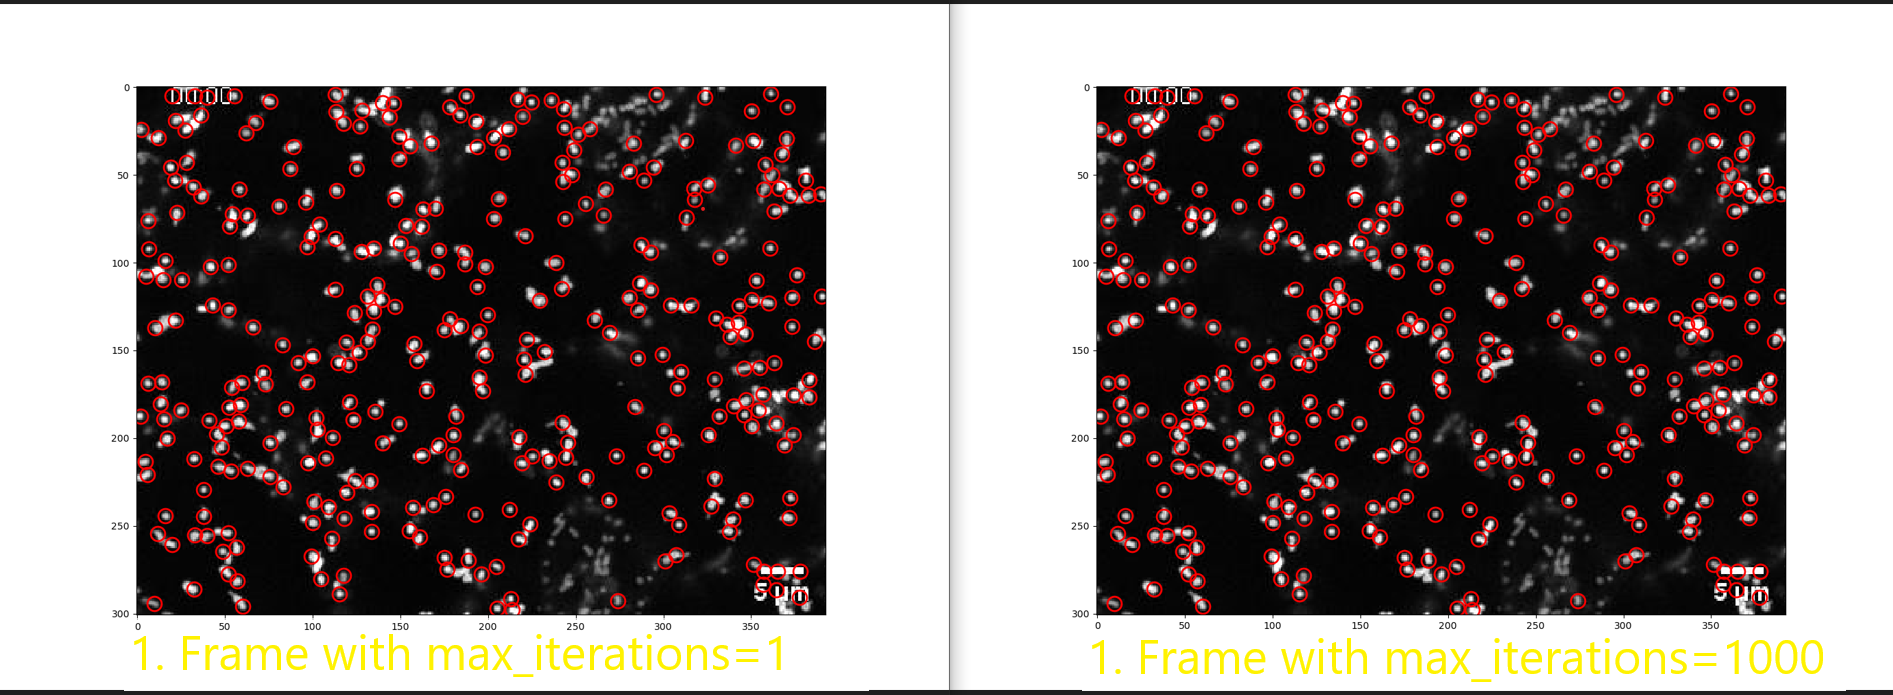
\includegraphics[scale=0.35]{Grafiken/trackpyBilder/comparison max_iterations.png}
    \caption{Vergleich zwischen max\_iterations=1 und max\_iterations=1000 auf demselben Frame.}
    \label{fig:comparison max-iterations}
\end{figure} 
	
\end{itemize}
